\documentclass[11pt,a4paper]{article}
\usepackage[margin=1in]{geometry}
\usepackage{amsmath,amssymb,bm}
\usepackage{graphicx}
\usepackage{booktabs}
\usepackage{hyperref}
\usepackage{siunitx}
\hypersetup{colorlinks=true,linkcolor=blue,citecolor=blue,urlcolor=blue}

\title{FYS5419 Project 1: VQE and the Lipkin Model}
\author{Your Name}
\date{Spring 2026}

\begin{document}
\maketitle

\begin{abstract}
This report studies one- and two-qubit Hamiltonians and the Lipkin model using classical diagonalization and a variational quantum eigensolver implemented from scratch. Replace this text with a concise summary of your final numerical findings.
\end{abstract}

\section{Introduction}
Explain the physical problem, the role of the interaction strength, and why VQE is relevant for small Hamiltonians written in terms of Pauli matrices.

\section{Methods}
Describe the state-vector simulator, measurements, density matrices, partial traces, von Neumann entropy, standard diagonalization, Pauli decompositions, and VQE ansatz choices.

\section{Part a: one-qubit gates and Bell states}
Discuss the action of $X$, $Y$, $Z$, $H$, and $S$ on $|0\rangle$ and $|1\rangle$. Discuss Bell-state preparation and the measured average outcomes. Include the reduced density matrix and entropy.

\section{Parts b--c: one-qubit Hamiltonian and VQE}
The Hamiltonian is
\[
H(\lambda)=H_0+\lambda H_I.
\]
Include the Pauli form and compare exact diagonalization with the one-parameter VQE.

\begin{figure}[h]
\centering
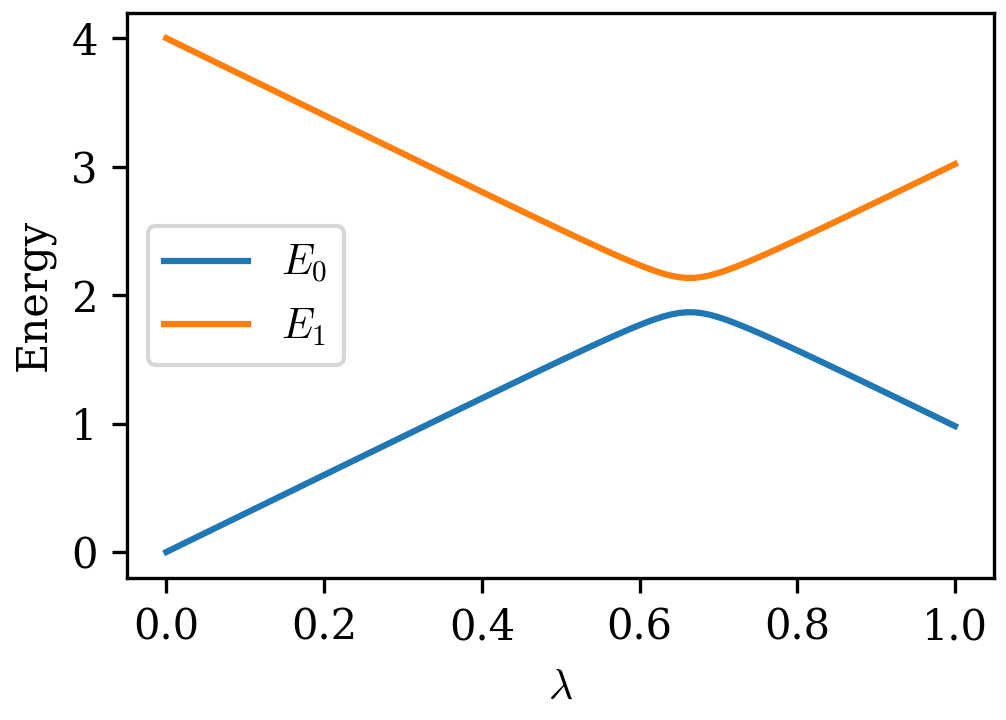
\includegraphics[width=0.72\linewidth]{../results/figures/part_b_one_qubit_eigenvalues.png}
\caption{Exact eigenvalues of the one-qubit Hamiltonian as functions of $\lambda$.}
\end{figure}

\begin{figure}[h]
\centering
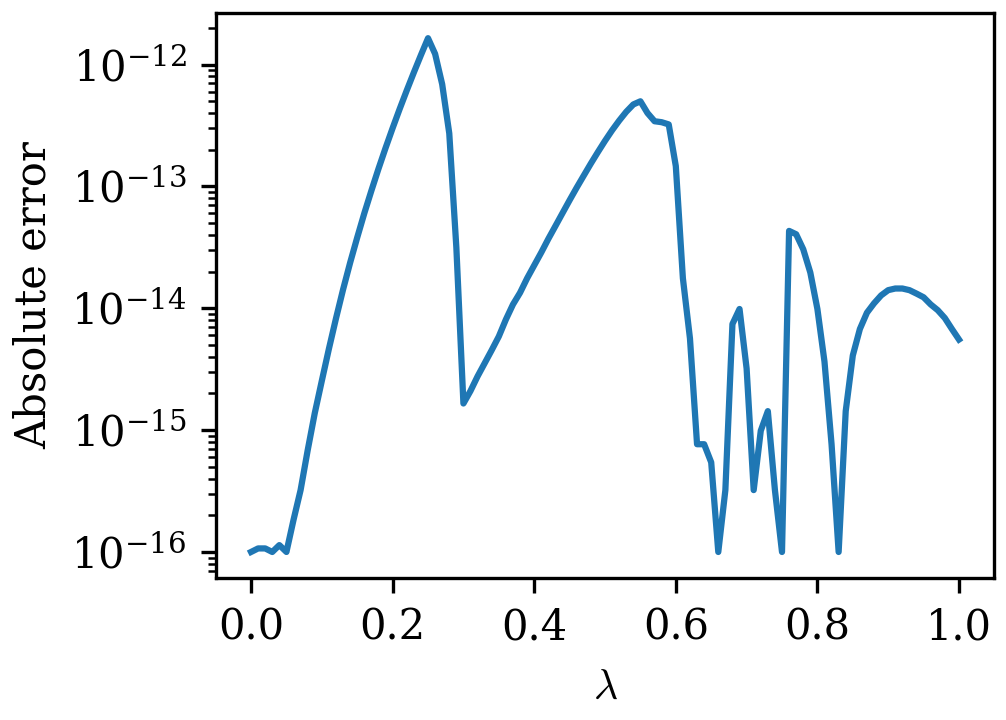
\includegraphics[width=0.72\linewidth]{../results/figures/part_c_one_qubit_vqe_error.png}
\caption{Absolute error of the one-qubit VQE ground-state energy.}
\end{figure}

\section{Parts d--e: two-qubit Hamiltonian, entanglement, and VQE}
Discuss the two-qubit Hamiltonian, exact eigenvalues, the reduced density matrix of the ground state, and the entropy $S(\rho_A)$.

\begin{figure}[h]
\centering
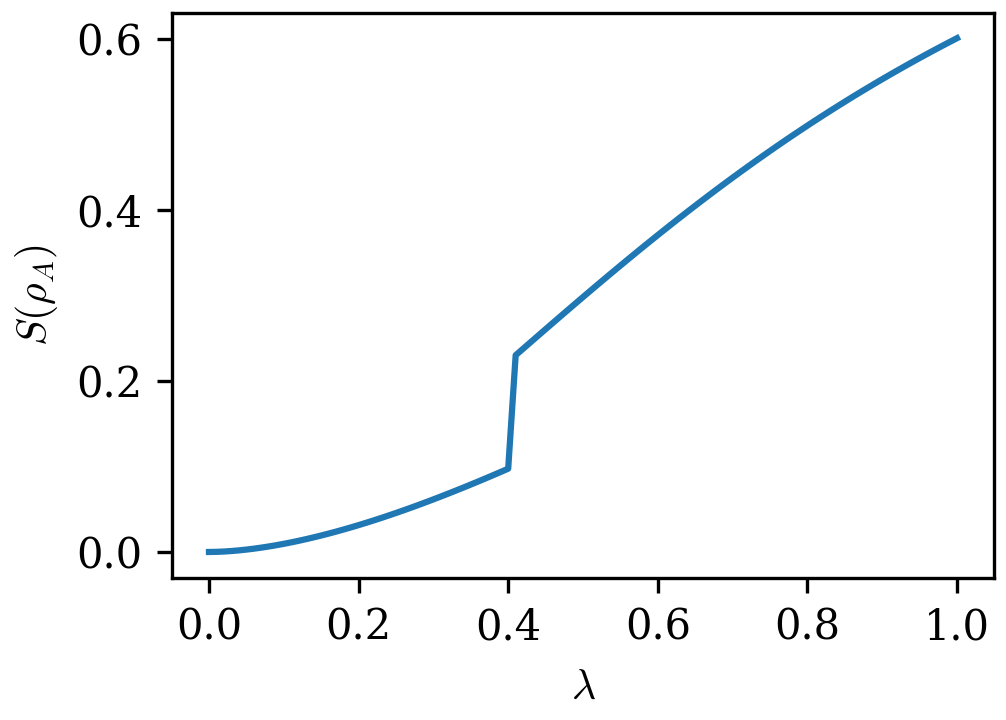
\includegraphics[width=0.72\linewidth]{../results/figures/part_d_two_qubit_entropy.png}
\caption{Ground-state entanglement entropy for subsystem $A$.}
\end{figure}

\section{Parts f--g: Lipkin model and VQE}
Present the $J=1$ and $J=2$ Lipkin Hamiltonians, their Pauli decompositions after padding to qubit Hilbert spaces, exact spectra, and VQE comparison.

\begin{figure}[h]
\centering
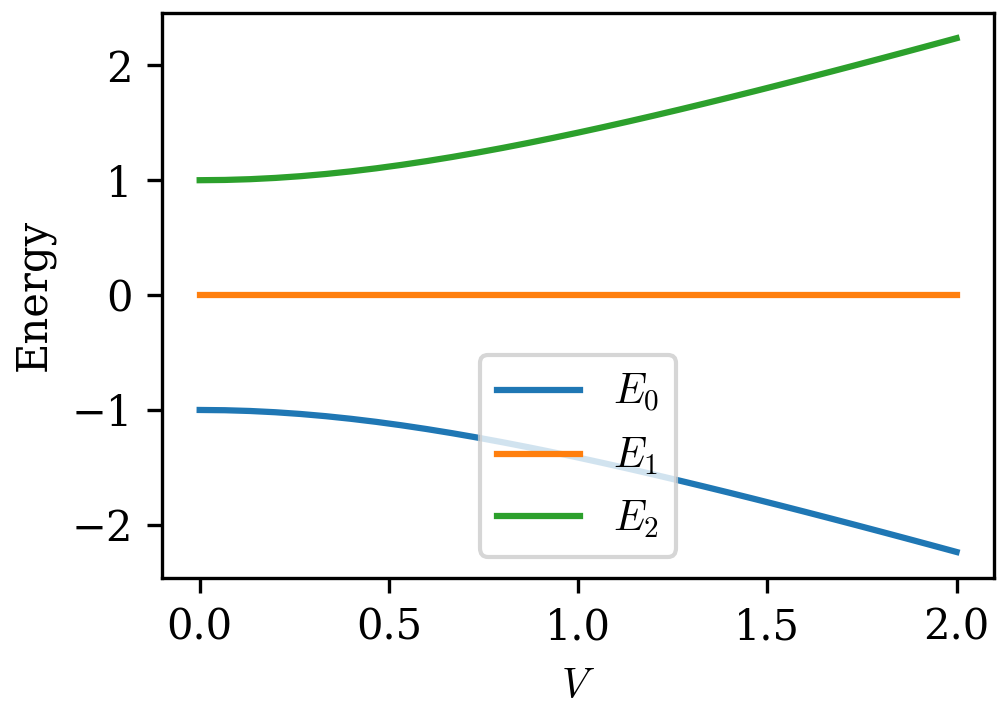
\includegraphics[width=0.72\linewidth]{../results/figures/part_f_lipkin_j1_exact.png}
\caption{Exact eigenvalues of the Lipkin $J=1$ Hamiltonian.}
\end{figure}

\begin{figure}[h]
\centering
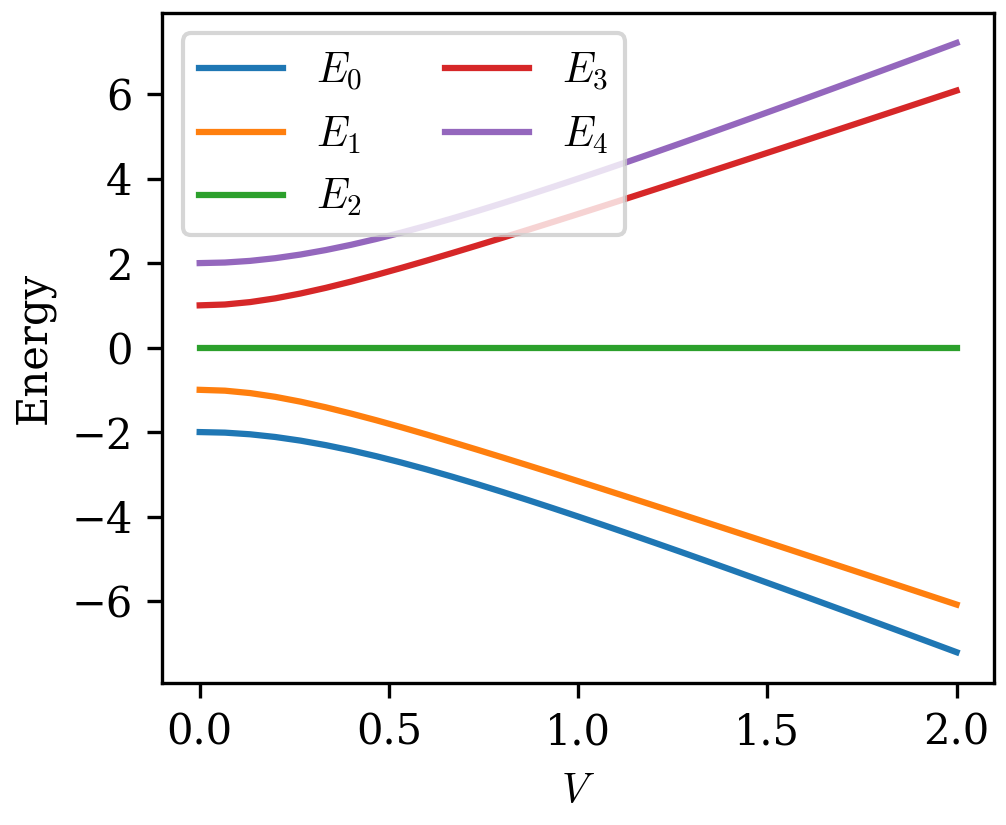
\includegraphics[width=0.72\linewidth]{../results/figures/part_f_lipkin_j2_exact.png}
\caption{Exact eigenvalues of the Lipkin $J=2$ Hamiltonian.}
\end{figure}

\begin{figure}[h]
\centering
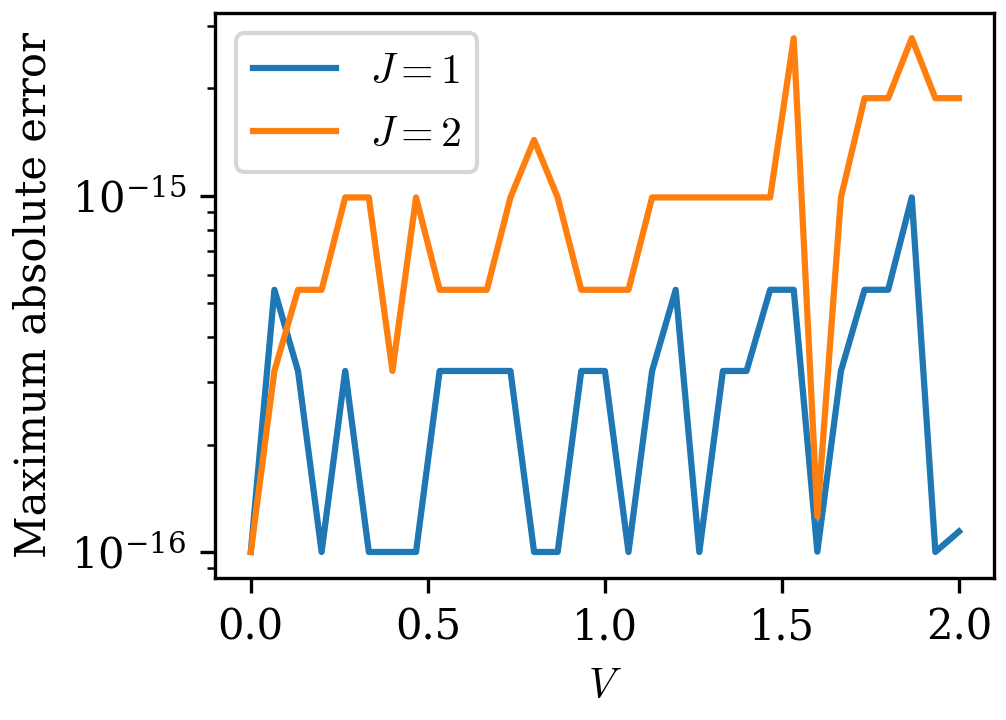
\includegraphics[width=0.72\linewidth]{../results/figures/part_g_lipkin_vqe_error.png}
\caption{VQE ground-state energy error for the embedded Lipkin Hamiltonians.}
\end{figure}

\section{Conclusion}
Summarize the main observations: level mixing, entanglement growth, VQE agreement with exact diagonalization, and limitations of the chosen ansatz.

\appendix
\section{Reproducibility}
The numerical results were generated with:
\begin{verbatim}
python scripts/run_all.py
\end{verbatim}

\section{AI/LLM declaration}
State clearly how AI tools were used, which parts were checked by you, and which calculations/results were generated by your own code.

\end{document}
